\chapter{Progettazione UML}

\section{Diagramma UML generale}

Il diagramma riportato nella Figura~\ref{fig:uml_general} mostra la
struttura complessiva del progetto, evidenziando le classi, i package di
appartenenza e le relazioni tra le classi.

\begin{figure}[H]
    \centering
    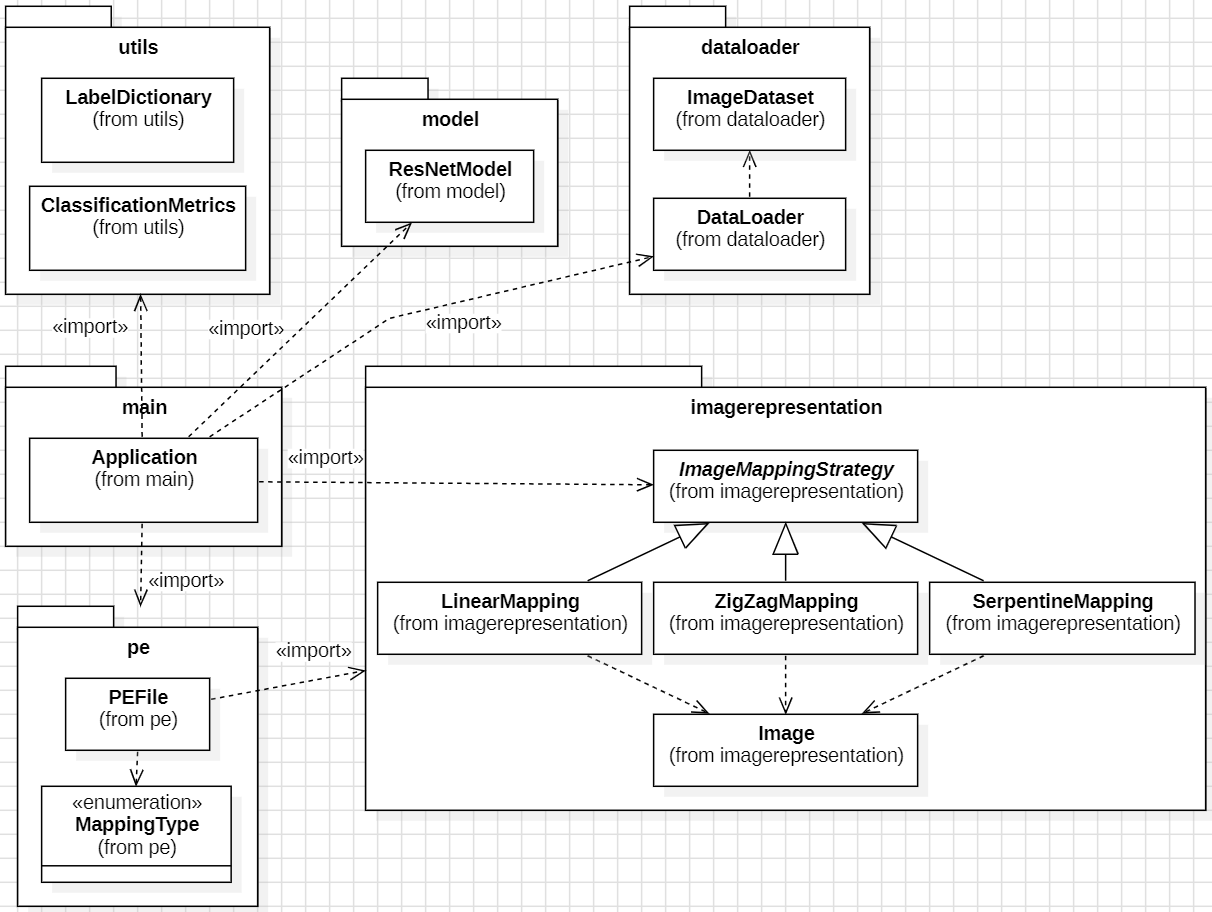
\includegraphics[width=0.971\textwidth]{images/uml_general.png}
    \caption{Diagramma UML generale del progetto}
    \label{fig:uml_general}
\end{figure}

\section{Package main}

Il package \texttt{main} (Figura~\ref{fig:package_main}) contiene il
punto di ingresso del programma e coordina l’esecuzione della pipeline.
Al suo interno vengono letti i parametri del file di configurazione e
vengono avviate le principali fasi del processo.

\begin{figure}[H]
    \centering
    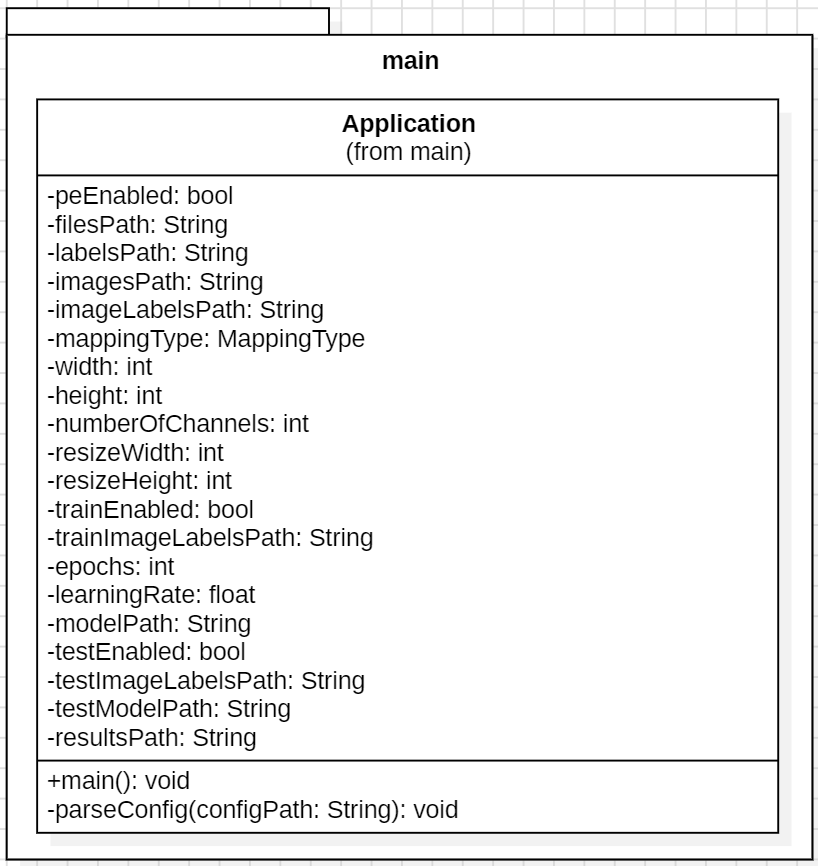
\includegraphics[width=0.85\textwidth]{images/package_main.png}
    \caption{Diagramma UML del package \texttt{main}}
    \label{fig:package_main}
\end{figure}

\subsection{Classe Application}

La classe \texttt{Application}, appartenente al package \texttt{main}, è
la classe principale del programma e si occupa di leggere il file di
configurazione e, in base ai parametri
impostati, di coordinarne le diverse fasi. Per svolgere le
varie operazioni, richiama le classi responsabili della conversione dei
file PE, della creazione del file CSV con le etichette, del training e
del test del modello. Durante la fase di test, coordina anche il calcolo
delle metriche e il salvataggio dei risultati.

\paragraph{Attributi}

\begin{itemize}
    \raggedright
    \item \textbf{peEnabled} (\texttt{bool}): indica se abilitare la fase di
    conversione PE in immagini.
    \item \textbf{filesPath} (\texttt{String}): percorso della cartella
    contenente i file PE da convertire.
    \item \textbf{labelsPath} (\texttt{String}): percorso del file CSV
    contenente i nomi dei file PE e le relative etichette.
    \item \textbf{imagesPath} (\texttt{String}): percorso della cartella in cui
    vengono salvate le immagini generate.
    \item \textbf{imageLabelsPath} (\texttt{String}): percorso del file CSV
    in cui viene salvato il mapping tra il percorso delle immagini generate e
    le relative etichette.
    \item \textbf{mappingType} (\texttt{MappingType}): strategia di mapping da
    utilizzare.
    \item \textbf{width} (\texttt{int}): larghezza delle immagini da generare.
    \item \textbf{height} (\texttt{int}): altezza delle immagini da generare.
    \item \textbf{numberOfChannels} (\texttt{int}): numero di canali
    delle immagini da generare.
    \item \textbf{resizeWidth} (\texttt{int}): larghezza per l'eventuale resize.
    \item \textbf{resizeHeight} (\texttt{int}): altezza per l'eventuale resize.
    \item \textbf{trainEnabled} (\texttt{bool}): indica se abilitare la fase di
    training del modello.
    \item \textbf{trainImageLabelsPath} (\texttt{String}): percorso del file CSV
    contenente il mapping immagini-etichette utilizzato durante il training.
    \item \textbf{epochs} (\texttt{int}): numero di epoche del training.
    \item \textbf{learningRate} (\texttt{float}): learning rate utilizzato
    durante il training.
    \item \textbf{modelPath} (\texttt{String}): percorso della cartella in cui
    viene salvato il modello addestrato.
    \item \textbf{testEnabled} (\texttt{bool}): indica se abilitare la fase di
    test del modello addestrato.
    \item \textbf{testImageLabelsPath} (\texttt{String}): percorso del file CSV
    contenente il mapping immagini-etichette utilizzato durante il test.
    \item \textbf{testModelPath} (\texttt{String}): percorso della cartella
    contenente il modello da utilizzare durante il test.
    \item \textbf{resultsPath} (\texttt{String}): percorso del file CSV in cui
    vengono salvati i risultati del test e le metriche calcolate.
\end{itemize}

\paragraph{Metodi}

\begin{itemize}
    \raggedright
    \item \textbf{main()} $\rightarrow$ \texttt{void}: punto di ingresso
    del programma. Coordina l’esecuzione delle diverse fasi in base ai
    parametri caricati dal file di configurazione.
    \item \textbf{parseConfig}(\texttt{configPath: String})
    $\rightarrow$ \texttt{void}: metodo
    privato che legge il file di configurazione e inizializza gli
    attributi necessari per l’esecuzione delle diverse fasi del programma.
\end{itemize}

\section{Package pe}

Il package \texttt{pe} (Figura~\ref{fig:package_pe}) si occupa della gestione dei file Portable
Executable di Windows. Il suo compito principale è leggere i file PE in
formato binario e avviare il processo di conversione in immagini,
utilizzando la strategia di mapping ricevuta dalla classe \texttt{Application}.

\begin{figure}[H]
    \centering
    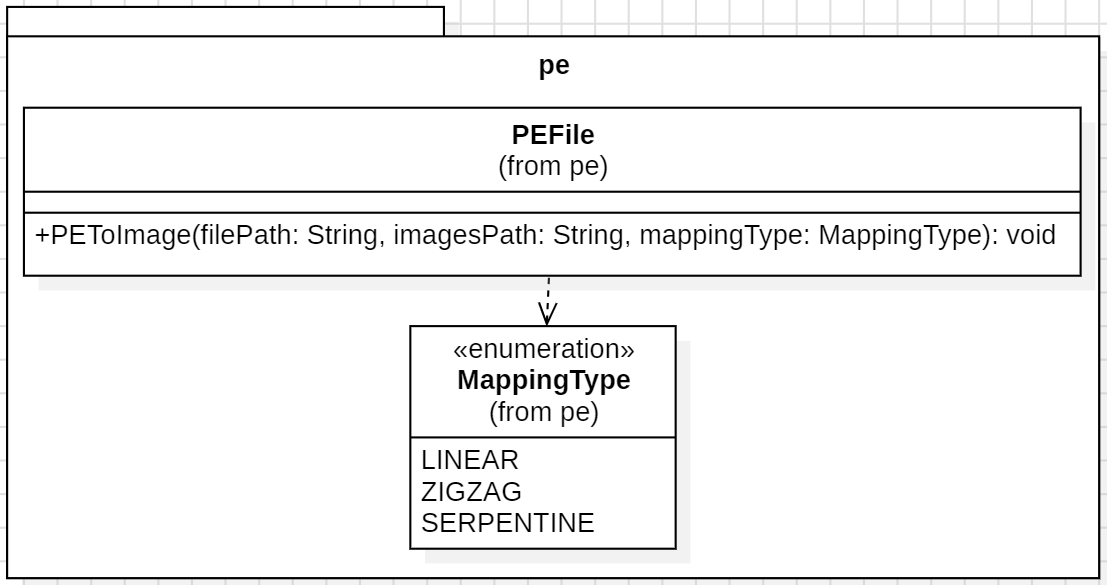
\includegraphics[width=\textwidth]{images/package_pe.PNG}
    \caption{Diagramma UML del package \texttt{pe}}
    \label{fig:package_pe}
\end{figure}

\subsection{Classe PEFile}

La classe \texttt{PEFile}, appartenente al package \texttt{pe}, è
responsabile della conversione di un singolo file PE. Riceve il percorso
del file, il percorso della cartella in cui
salvare l’immagine e il valore di \texttt{MappingType}. Dopo aver letto il
contenuto binario del file, utilizza il tipo di mapping ricevuto per
individuare la strategia da applicare e salva infine l’immagine generata
nella cartella specificata.

\paragraph{Metodi}

\begin{itemize}
    \raggedright
    \item \textbf{PEToImage}(\texttt{filePath:String},
    \texttt{imagesPath:String}, \texttt{mappingType:MappingType})
    $\rightarrow$ \texttt{void}: legge il singolo file PE indicato,
    genera l’immagine utilizzando la strategia di mapping ricevuta e salva
    il risultato nella cartella delle immagini specificata.
\end{itemize}

\subsection{Enumerazione MappingType}

L’enumerazione \texttt{MappingType}, appartenente al package \texttt{pe},
definisce il tipo di strategia di mapping da utilizzare per la conversione
dei file PE in immagini. Il valore viene letto dal file di configurazione
dalla classe
\texttt{Application} e passato alla classe
\texttt{PEFile}, che lo utilizza per determinare la strategia di mapping
da applicare durante la generazione delle immagini.

\paragraph{Valori}

\begin{itemize}
    \raggedright
    \item \textbf{LINEAR}
    \item \textbf{ZIGZAG}
    \item \textbf{SERPENTINE}
\end{itemize}

\section{Package image\_representation}

Il package \texttt{image\_representation} contiene le funzionalità
necessarie per la conversione dei file PE in immagini. Al suo interno
sono definite le diverse strategie di mapping utilizzate per disporre i
byte del file nell’immagine.

\begin{figure}[H]
    \centering
    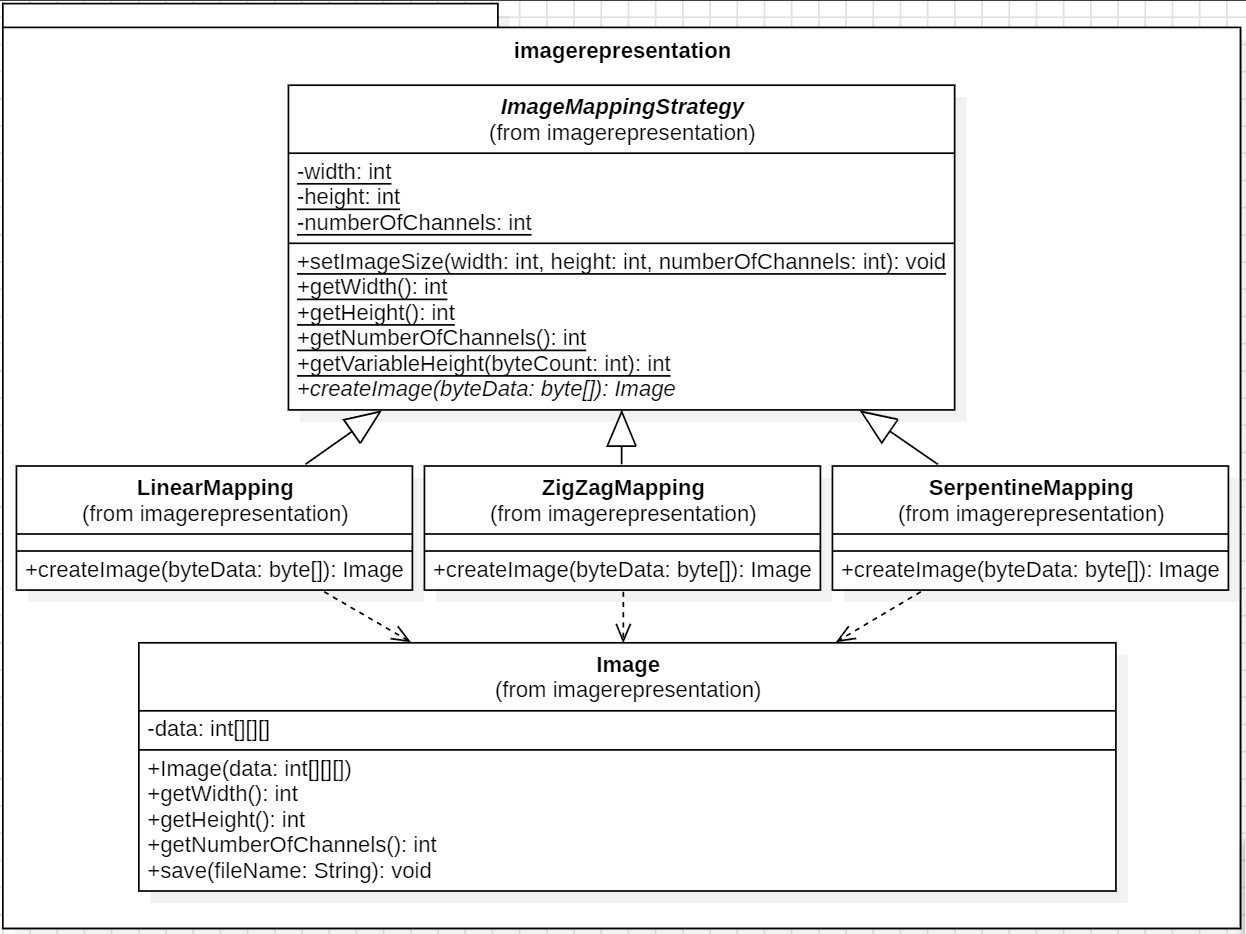
\includegraphics[width=\textwidth]{images/package_imagerepresentation.PNG}
    \caption{Diagramma UML del package \texttt{image\_representation}}
    \label{fig:package_image_representation}
\end{figure}

\subsection{Classe Image}

La classe \texttt{Image}, appartenente al package
\texttt{image\_representation}, rappresenta l’immagine finale ottenuta
dalla conversione del file PE. L’immagine è rappresentata tramite un tensore a
tre dimensioni che contiene i valori dei pixel organizzati secondo righe,
colonne e canali. La classe riceve il tensore già costruito dalla strategia
di mapping e si occupa della sua gestione e del salvataggio su file.

\paragraph{Attributi}

\begin{itemize}
    \raggedright
    \item \textbf{data} (\texttt{int[][][]}): tensore tridimensionale che
    contiene i valori dell’immagine organizzati in altezza, larghezza e
    numero di canali.
\end{itemize}

\paragraph{Metodi}

\begin{itemize}
    \raggedright
    \item \textbf{Image}(\texttt{data:int[][][]}): costruttore della classe
    che inizializza l’immagine.
    \item \textbf{getWidth}() $\rightarrow$ \texttt{int}: restituisce la
    larghezza dell’immagine ricavandola dal tensore associato.
    \item \textbf{getHeight}() $\rightarrow$ \texttt{int}: restituisce
    l’altezza dell’immagine ricavandola dal tensore associato.
    \item \textbf{getNumberOfChannels}() $\rightarrow$ \texttt{int}:
    restituisce il numero di canali dell’immagine ricavandola dal tensore
    associato.
    \item \textbf{save}(\texttt{fileName:String}) $\rightarrow$
    \texttt{void}: salva l’immagine su file.
\end{itemize}

\subsection{Classe astratta ImageMappingStrategy}

La classe astratta \texttt{ImageMappingStrategy} definisce il comportamento
comune delle strategie di mapping. Appartiene al package
\texttt{image\_representation}. Contiene i parametri necessari alla
costruzione dell’immagine, cioè larghezza, altezza e numero di canali,
impostati prima della fase di creazione dell’immagine. Ogni implementazione
riceve in input la sequenza di byte del file PE e costruisce l’immagine
utilizzando un diverso ordine di inserimento dei dati in base alla strategia
scelta.
L’altezza può essere definita nel file di configurazione oppure impostata a
0 per utilizzare la modalità a altezza variabile. In questo caso, l’altezza
necessaria viene calcolata durante la creazione dell’immagine senza
modificare la configurazione della strategia.
La gestione dei canali permette di costruire immagini sia in grayscale
(1 canale) sia RGB (3 canali), modificando la granularità con cui i byte
vengono letti e inseriti nel tensore, in particolare un byte per pixel nel
caso grayscale oppure gruppi di tre byte per pixel nel caso RGB.

\paragraph{Attributi}

\begin{itemize}
    \raggedright
    \item \textbf{width} (\texttt{int}, statico): larghezza comune
    utilizzata per la costruzione delle immagini.
    \item \textbf{height} (\texttt{int}, statico): altezza comune
    utilizzata per la costruzione delle immagini.
    \item \textbf{numberOfChannels} (\texttt{int}, statico): numero di
    canali utilizzato per definire la struttura del tensore.
\end{itemize}

\paragraph{Metodi}

\begin{itemize}
    \raggedright
    \item \textbf{setImageSize}(\texttt{width:int}, \texttt{height:int},
    \texttt{numberOfChannels:int}) $\rightarrow$ \texttt{void}
    (statico): imposta i parametri comuni utilizzati dalle strategie per
    costruire l’immagine.
    \item \textbf{getVariableHeight}(\texttt{byteCount:int})
    $\rightarrow$ \texttt{int} (statico): calcola e restituisce l’altezza
    necessaria in base alla dimensione del file quando l’altezza non è
    definita.
    \item \textbf{getWidth}() $\rightarrow$ \texttt{int} (statico):
    restituisce la larghezza configurata.
    \item \textbf{getHeight}() $\rightarrow$ \texttt{int} (statico):
    restituisce l’altezza configurata.
    \item \textbf{getNumberOfChannels}() $\rightarrow$ \texttt{int}
    (statico): restituisce il numero di canali configurato.
    \item \textbf{createImage}(\texttt{byteData:byte[]}) $\rightarrow$
    \texttt{Image} (astratto): costruisce e restituisce l’immagine a partire
    dai byte del file PE.
\end{itemize}

\subsection{Classe LinearMapping}

La classe \texttt{LinearMapping}, appartenente al package
\texttt{image\_representation}, implementa il mapping inserendo i byte nel
tensore in modo sequenziale, da sinistra verso destra e dall’alto
verso il basso.

\paragraph{Metodi}

\begin{itemize}
    \raggedright
    \item \textbf{createImage}(\texttt{byteData:byte[]}) $\rightarrow$
    \texttt{Image}: costruisce l’immagine utilizzando il mapping lineare.
\end{itemize}

\subsection{Classe ZigZagMapping}

La classe \texttt{ZigZagMapping}, appartenente al package
\texttt{image\_representation}, implementa il mapping alternando la
direzione di riempimento delle righe, seguendo un andamento a zigzag.

\paragraph{Metodi}

\begin{itemize}
    \raggedright
    \item \textbf{createImage}(\texttt{byteData:byte[]}) $\rightarrow$
    \texttt{Image}: costruisce l’immagine utilizzando il mapping a zigzag.
\end{itemize}

\subsection{Classe SerpentineMapping}

La classe \texttt{SerpentineMapping}, appartenente al package
\texttt{image\_representation}, implementa il mapping seguendo un
andamento a serpentina.

\paragraph{Metodi}

\begin{itemize}
    \raggedright
    \item \textbf{createImage}(\texttt{byteData:byte[]}) $\rightarrow$
    \texttt{Image}: costruisce l’immagine utilizzando il mapping a
    serpentina.
\end{itemize}
